Dieses Kapitel bietet einen Überblick über einige p2p-Netzwerke und evaluiert diese anhand gestellter Anforderungen. Diese Evaluierung beeinflußt die Entscheidung für ein Overlay-Netzwerk auf das schließlich, das in dieser Arbeit zu entwickelnde, generische Publish/Subscribe-System gesetzt wird. Die Evaluierung bedient sich zahlreicher Arbeiten, die sich alleine dem Vergleich dieser Netzwerke widmen \cite{Lua2005Survey, Goetz2005, Li2004Comparing, Darlagiannis2006Peertopeer, Castro2002Secure, Bo2003PeertoPeer} und geht auch auf ihre Nutzbarkeit als Basis für \emph{Application level multicast} sprich ein Publish/Subscribe-System ein \cite{Hosseini2007Survey, Fahmy2007, Castro2003Evaluation, Ratnasamy2001}.

Zuvor müssen jedoch die eigenen Anforderungen an solche Systeme identifiziert werden. Zu den offensichtlichen Anforderungen wie beispielsweise \emph{Skalierbarkeit} gesellen sich jedoch auch spezielle Anforderungen aus Spielsicht hinzu. Diese sind beispielsweise das Vorhandensein eines Masterservers oder das Übertragen von Applikationswissen auf das Netzwerk um damit dessen Entscheidungen bezüglich Nachbarschaften oder Versand von Nachrichten (Routing) zu beeinflussen.

\section{Anforderungen}

\paragraph{Geringe Latenz} Schnelle Reaktionszeiten und Nachrichtenübermittlung sind bei \ac{mmog} unverzichtbar. Ebenfalls müssen größere Nachrichten (beispielsweise Update der Welt) schnell übertragen werden damit der Spielfluss nicht behindert wird. Dies lässt sich anhand der Anzahl der Hops beim Nachrichtenversand messen.

\paragraph{Skalierbar} Selbst bei einer großen Anzahl an Knoten soll das Netz nicht kollabieren. Hierbei ist es auch wichtig, dass Knoten nicht unbedingt lange im Spiel sein müssen. Zwar kann davon ausgegangen werden, dass ein durchschnittlicher Spieler längere Zeit im Spiel verbringt, aber durch Netzausfälle oder sonstigen Unbill kann dies stark variieren. Insofern ist es wichtig wie sich die Netzwerke bei großen Fluktationen verhalten \cite{Li2004Comparing}.

\paragraph{Fehlertoleranz bei Knotenausfall} Fallen Knoten aus, muss sich das Netz ohne großen Kommunikationsaufwand selbst reparieren. Ebenfalls mögliche Netzwerkpartitionierungen sind in dieser Arbeit jedoch kein Hindernis, denn der Hauptserver kann über eine gesonderte Verbindung immer erreicht werden. Damit kann das Netz wieder verbunden werden.\\
Interessant hierbei ist auch die eingebaute Redundanz einiger Systeme, die Daten auf mehrere Knoten verteilen. Wie sich dies im Vergleich von statischen Daten zu sich häufig verändernden Objekten der Spielewelt verhält ist zu untersuchen. 

\paragraph{Kommunikation über das Netzwerk} Das Netzwerk soll nicht nur das schnelle Auffinden von Peers ermöglichen, sondern auch einen Transport der Nachricht (Routing) durch das Netzwerk selbst bereitstellen. Die Alternative Direktverbindungen soll nur genutzt werden, wenn eine Datenübertragung im Netzwerk nicht performant genug ist, weil z.B. die Bandbreite der zwischengeschalteten Peers zu gering ist.

\paragraph{Bestimmung der Nachbarschaft} Eine dynamische Bestimmung der Nachbarschaftsgröße kann von Vorteil sein. So könnten Knoten mit mehr Bandbreite (bzw. entsprechenden anderen Metriken) mehr direkte Verbindungen halten als Knoten mit geringer Bandbreite (oder geringer Spieldauer).

\paragraph{Eingriff in Routingentscheidungen} Applikationswissen hilft auch beim Eingriff in das Routing des Netzes. So können Knoten bevorzugt zur Weiterleitung einer Nachricht ausgewählt werden. Diese Knoten zeichnen sich beispielsweise durch eine große Bandbreite oder spezielle Applikationsmetriken\footnote{Bsp: Spieler befindet sich in der selben Stadt} aus.

\paragraph{Verfügbarkeit als C/C++-Bibliothek} Da der Prototyp dieser Arbeit sowie das Umfeld in C++ entwickelt wird, gibt es damit eine weitere Anforderung an das Netzwerk: Die Verfügbarkeit als C/C++-Bibliothek.\\
Damit ist das Netzwerk einfach aus bestehendem Code nutzbar ohne dass kostenintensive Brücken zwischen beispielsweise Java und C++ geschlagen werden müssen. Da zudem betriebssystemübergreifend\footnote{In unserem Fall auf Windows und Linux} entwickelt und getestet wird, ist außerdem ein zur Verfügung stehender Quellcode vorteilhaft. Nur dadurch ist es möglich eventuellen betriebsystembezogenen Netzwerk- oder Threadcode auf  Boost\footnote{Zahlreiche Bibliotheken für C++: http://www.boost.org} zu portieren um somit eine betriebsystemübergreifende Benutzung zu ermöglichen.

\paragraph{Unterbau eines Publish/Subscribe-Systems} Das Overlay-Netzwerk muss so gestaltet sein, dass es dem Anwendungsfall \emph{Application level multicast} genügt und dessen besondere Anforderungen (auch von Spielseite)\footnote{siehe Kapitel \ref{chap:evaluation_pubsub}} her unterstützt.

Anhand dieser Anforderungen sind unstrukturierte Netzwerke nicht als Netzwerksystem für dieser Arbeit geeignet. Eine Suche, bzw. Datenübertragung durch Flooding widerspricht klar der Anforderung nach geringer Latenz. Ebenso sind diese Netzwerke auf eine Übertragung via Direktverbindung ausgelegt.

\cite{Dabek2003Towards} stellt eine generische \ac{api} für \ac{kbr} Systeme vor, wie es viele der strukturierten Netzwerke anbieten vor und zeigt wie darauf aufbauen verschiedene Systeme wie \ac{dht}, \ac{dolr} und \ac{cast}\footnote{entspricht Application level multicast} implementiert werden können. Ebenfalls wird gezeigt wie einige bekannte Systeme (CAN, Chord, Pastry und Tapestry) diese die Anforderungen erfüllen.\\
Daraus ergibt sich eine weitere spezielle Anforderung an das Overlay-Netzwerk:

\paragraph{Anpassbarkeit an generische \ac{api}} Lässt sich das Netzwerk der genersischen \ac{api} anpassen, gewinnt das an Flexibiliät, da die Netzwerkschicht ohne große Änderungen an den restlichen Systemschichten ausgetauscht und verändert werden kann.

\section{generic API}
\label{chap:evaluation_p2p:generic_api}
\cite{Dabek2003Towards} %towards

\lstinputlisting[caption={Upcalls der generischen API}, label=code:towards_upcall]{listings/towards_upcall.cpp}



\section{Evaluation}
In diesem Kapitel werden die vier bekannten Systeme Chord \cite{Stoica2003}, Pastry \cite{Rowstron2001}, Tapestry \cite{Zhao2001Tapestry,Zhao2004Tapestry} und CAN \cite{Ratnasamy2001Scalable} miteinander verglichen. Die ersten drei sind in ihrem Aufbau ähnlich (Schlüsselraum wird auf einen Ring verteilt) und unterscheiden sich in der Art des Routings. CAN hingegeen bildet den Schlüsselraum auf ein d-dimensionalen kartesisches Koordinatensystem ab. Alle vier Systeme sind laut \cite{Dabek2003Towards} im Hinblick auf die generische \ac{api} nutzbar.

Zur Entscheidungsfindung werden die Netzwerke anhand folgender Gesichtspunkt verglichen:
\begin{itemize}
\item Aufbau und Struktur
\item Routing
\item Nachbarschaft
\item Eintritt und Austritt (Fehlerfall) von Knoten
\item Nutzbarkeit als Basis für \ac{cast}
\end{itemize}

\subsection{Aufbau und Struktur}
Bei Chord \cite{Stoica2003} sind die l-bit wertigen Schlüssel (meist Zahlen im Bereich $[0,2^l-1]$) auf einem eindimensionalen Ring modulo $2^l$ im Uhrzeigersinn angelegt. Jedem Knoten und jedem Datum ist ein eindeutiger Schlüssel zugewiesen, diese sind \emph{ID} und \emph{key} benannt. Jeder Schlüssel (und damit jeder Knoten und jedes Datum) besitzt einen Vorgänger und einen Nachfolger. Der Vorgänger von $X$ ist derjenige erste Schlüssel entgegen dem Uhrzeigersinn, dessen ID kleiner ist als ID von $X$ und wird $PRED(X)$ benannt. Ensprechend ist der Nachfolger $SUCC(X)$ der erste Schlüssel im Uhrzeigersinn, dessen ID größer gleich der ID von $X$ ist.

\begin{figure}[htb]
\centering
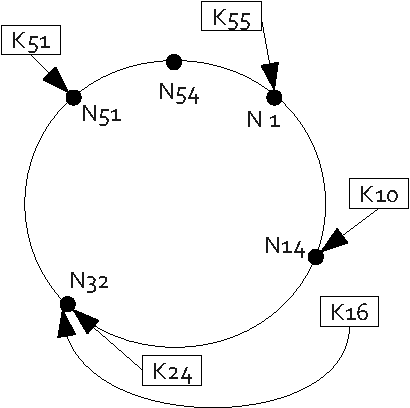
\includegraphics{grafics/chord_key_space.pdf}
\caption{a) Schlüsselraum ($l=6$) für Chord mit sechs Knoten und fünf Daten b) Fingertabelle für Knoten $N1$ }
\label{fig:chord_key_space}
\end{figure}

Ein Knoten $A$ ist dabei für alle Daten zuständig die zwischen $A$ und $PRED(A)$ liegen, somit gilt: $$PRED(A) < key(Datum) \le ID_A$$
In Figur \ref{fig:chord_key_space} a) ist dies bildlich für sechs Knoten und fünf Datenpunkten bei $l=6$ gezeigt. Knoten 14 (N14) ist für das Datum mit Schlüssel 10 (K10) zuständig. Knoten 32 ist für K16 und K25. K51 ist bei N51 zu finden. Aufgrund der Ringstruktur ist N1 für K55 zuständig.

\subsection{Routing}
Bei Chord besitzt jeder Knoten eine Verbindung zu seinem direkten Vorgänger und seinem direkten Nachfolger. Weiterhin pflegt jeder Knoten eine sogenannte \emph{finger table}. Die maximal $l$ Einträge in dieser Tabelle zeigen auf andere Knoten im Ring, so dass der Eintrag in Zeile $i$ von Knoten $n$ denjenigen Knoten enthält der $n$ mit mindestens $2^{i-1}$ folgt. Figur \ref{fig:chord_key_space} b) stellt die Fingertabelle von Knoten $N1$ dar. Die ersten Einträge $SUCC(2), SUCC(3) und SUCC(5)$ verweisen auf Knoten $N5$. Der dritte Eintrag verweist auf $SUCC(9) = N14$.

\subsection{Nachbarschaft}

\subsection{Eintritt und Austritt (Fehlerfall) von Knoten}

\subsection{Nutzbarkeit als Basis für \ac{cast}}

We also show that multicast trees built using Pastry provide higher performance than ones built using CAN \cite{Castro2003Evaluation, KostasKatrinis2005}.

\subsection{Fazit}

Aufgrund der mageren Ergebnisse in Castros Untersuchung \cite{Castro2003Evaluation} bleibt CAN trotz interessanter Ideen außen vor. Ebenso kann Chord nicht in Betracht gezogen werden, da es kurzzeitige Inkonsistenzen in der Nachbarschaft (und damit dem Routing) geben kann. Weiterhin wird eine größere Latenz im Nachrichtenversand erwartet, da Nachrichten nur in einer Richtung auf dem Ring weitergeleitet werden.

Pastry und Tapestry zeigen durch die Implementierung von Scribe und Bayeux \cite{Castro2002Scribe, Zhuang2001} dass sie als Unterbau für \ac{cast} sehr wohl geeignet sind. Pastry ist jedoch nur als Javabibliothek\footnote{http://www.freepastry.org} verfügbar und die Entwicklung von Tapestry (ebenfalls in Java implementiert) wurde mit Version 2.01 eingestellt.

Chimera ist der Nachfolger von Tapestry und vereint laut Homepage\footnote{http://current.cs.ucsb.edu/projects/chimera/index.html} das Beste von Pastry und Tapestry in sich: 

\begin{quote}
Chimera is a light-weight C implementation of a \emph{next-generation} structured overlay that provides similar functionality as prefix-routing protocols Tapestry and Pastry.  Chimera gains simplicity and robustness from its use of Pastry's leafsets, and efficient routing from Tapestry's locality algorithms.  In addition to these properties, Chimera also provides efficient detection of node and network failures, and reroutes messages around them to maintain connectivity and throughput.  
\end{quote}

Der frei verfügbare Code (veröffentlicht unter GPL), die Anpassbarkeit und die Unterstützung der Zielplatformen Linux und Windows sprechen stark für Chimera als Netzwerkunterbau für das in dieser Arbeit zu entwickelnde generische Publish/Subscribe-System.\\
Da Chimera der generischen \ac{api} entspricht, könnte es bei gravierenden Problemen durch ein anderes System ausgetauscht werden, ohne das restliche System zu beeinflussen.
